\documentclass[../../../main.tex]{subfiles}

\begin{document}
	\begin{figure}[h!]
        \centering
        \tikzset{every picture/.style={line width=0.75pt}} %set default line width to 0.75pt
        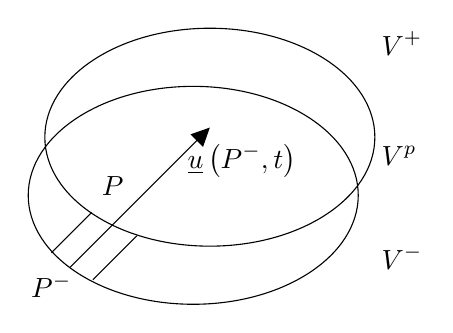
\begin{tikzpicture}[x=0.75pt,y=0.75pt,yscale=-1,xscale=1]
            %uncomment if require: \path (0,300); %set diagram left start at 0, and has height of 300
            %Shape: Ellipse [id:dp07065825847986607] 
            \draw   (17.82,94.32) .. controls (17.82,65.32) and (53.41,41.82) .. (97.32,41.82) .. controls (141.22,41.82) and (176.82,65.32) .. (176.82,94.32) .. controls (176.82,123.31) and (141.22,146.82) .. (97.32,146.82) .. controls (53.41,146.82) and (17.82,123.31) .. (17.82,94.32) -- cycle ;
            %Shape: Ellipse [id:dp8955108338689244] 
            \draw   (25.82,66.32) .. controls (25.82,37.32) and (61.41,13.82) .. (105.32,13.82) .. controls (149.22,13.82) and (184.82,37.32) .. (184.82,66.32) .. controls (184.82,95.31) and (149.22,118.82) .. (105.32,118.82) .. controls (61.41,118.82) and (25.82,95.31) .. (25.82,66.32) -- cycle ;
            %Straight Lines [id:da49541421749518166] 
            \draw    (38,129) -- (103.2,63.8) ;
            \draw [shift={(105.32,61.68)}, rotate = 135] [fill={rgb, 255:red, 0; green, 0; blue, 0 }  ][line width=0.08]  [draw opacity=0] (8.93,-4.29) -- (0,0) -- (8.93,4.29) -- cycle    ;
            %Straight Lines [id:da8429865237476364] 
            \draw    (29,122) -- (48.4,102.6) ;
            %Straight Lines [id:da29073454377070784] 
            \draw    (49,135) -- (70.2,113.8) ;
            % Text Node
            \draw (186.82,69.32) node [anchor=north west][inner sep=0.75pt]   [align=left] {$\displaystyle \mathscr{V}^p$};
            % Text Node
            \draw (186.82,14.32) node [anchor=north west][inner sep=0.75pt]   [align=left] {$\displaystyle \mathscr{V}^{+}$};
            % Text Node
            \draw (18,131) node [anchor=north west][inner sep=0.75pt]   [align=left] {$\displaystyle P^{-}$};
            % Text Node
            \draw (52,84) node [anchor=north west][inner sep=0.75pt]   [align=left] {$\displaystyle P$};
            % Text Node
            \draw (186.82,117.32) node [anchor=north west][inner sep=0.75pt]   [align=left] {$\displaystyle \mathscr{V}^{-}$};
            % Text Node
            \draw (93.32,68.68) node [anchor=north west][inner sep=0.75pt]   [align=left] {$\displaystyle \underline{u}\left( P^{-} ,t\right)$};
            \end{tikzpicture}
        \caption{Thể tích vật chất được xem xét để tính đạo hàm hạt là thể tích $\mathscr{V}$, ở thời điểm $t$ nó là phần hình bao ở phía dưới, ở thời điểm $t+\delta t$ nó là phần hình bao ở phía trên. Phần giao nhau giữa hai hình bao, $\mathscr{V}^p$, chính là phần thể tích cố định giữa hai thời điểm khảo sát; còn hai phần hình bán nguyệt là phần thể tích lưu chất đã bị dịch chuyển mà ta kí hiệu là $\mathscr{V}^+$ và $\mathscr{V}^-$. Điểm $P^-$ nằm trên bề mặt có vận tốc ở thời điểm $t$ là $\underline{u}(P^-,t)$ đã bị dịch chuyển thành điểm $P$ cũng nằm trên bề mặt.}
        \label{fig:Derivatie_Particulaire_Volumique}
    \end{figure}
\end{document}